\chapter{Introduction}
% ------------------------

\section{Aim and Background}
The aim of this project was to design an automated chip tester for the University
of Southampton Superchip, also known as D2. Undergraduates at the School of Electronics
and Computer Science participate every year in a project in which they
design a part of a digital chip. Figure \ref{fig:chip_overview} shows an overview
of the final chip, which includes up to 16 individual designs.
\begin{figure}[h!]
\centering
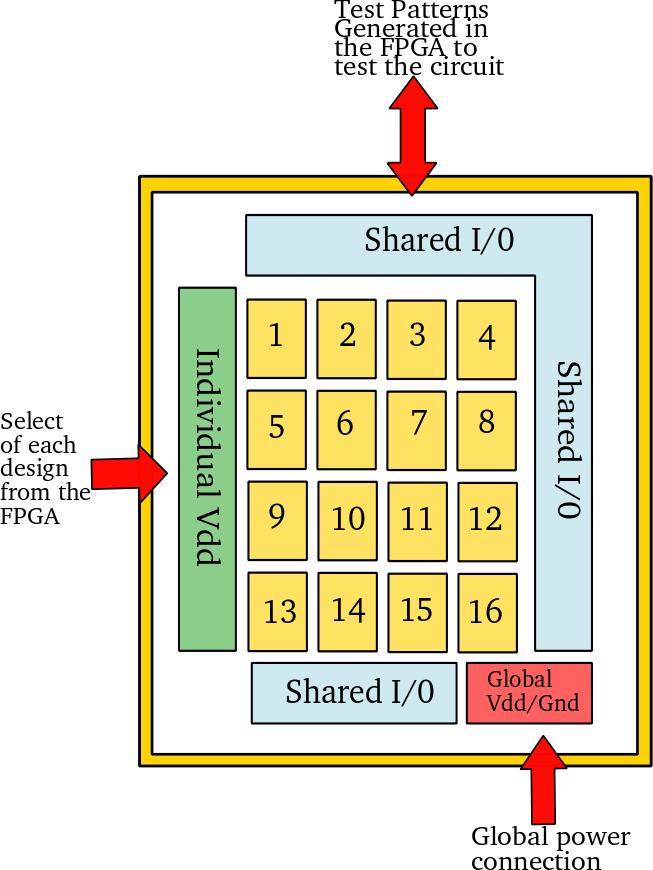
\includegraphics[scale=0.35]{Chip.png}
\caption{Overview of the Superchip (D2)}
\label{fig:chip_overview}
\end{figure}

All individual designs share the same 24 input and 24 output pins, but have separate power supplies.
As all of them share the same outputs, only one design can be active at any one time.
\\

Each of the 16 individual blocks on the chip is made up of smaller designs such as
adders, ring oscillators and other simple digital circuits. Every year one of the
smaller designs is an oscillator. As such, one of the requirements of the chip tester
is to measure the frequency of the on-chip oscillator.
\\

The chip tester was to be implemented using an Altera DE2-115 Development Board,
featuring an Altera Cyclone IV EP4CE115 FPGA.


\newpage
\section{DE2 Board Overview}
The DE2 board is an FPGA board designed by Terasic, based around an Altera
Cyclone IV FPGA. The following hardware relevant to this project is provided on
the DE2-115 board:

\begin{itemize}
 \item Altera Cyclone® IV EP4CE115 FPGA device 
 \item USB Blaster (on board) for programming; both JTAG and Active Serial (AS) programming modes are supported 
 \item 2MB SRAM (organized as 1M x 16 bits)
 \item 128MB SDRAM
 \item 8MB CFI Flash memory
 \item SD Card socket
 \item 50MHz oscillator
 \item 2 Gigabit Ethernet PHY with RJ45 connectors 
 \item RS-232 transceiver and 9-pin connector 
 \item One 40-pin Expansion Header with diode protection 
 \item One High Speed Mezzanine Card (HSMC) connector 
 \item 16x2 Character LCD display
\end{itemize}




\section{System Overview}
Pavlos (get started) \\
see slides